\documentclass{beamer}

\usepackage{amsmath}
\usepackage{amssymb}
\usepackage{amsthm}
\usepackage[UKenglish]{babel}
\usepackage{enumerate}
\usepackage{graphicx}
\usepackage{braket}
\usepackage{esint}
\usepackage{float}
\usepackage{tabularx}
\usepackage{array}
\usepackage{subcaption}
\usepackage{hyperref}
\hypersetup{colorlinks=false, bookmarks=true}

\usetheme{Madrid}
\usecolortheme{seahorse}
\usefonttheme{professionalfonts}
\useinnertheme{circles}

\AtBeginSection[]
{
  \begin{frame}
    \frametitle{Table of Contents}
    \tableofcontents[currentsection]
  \end{frame}
}

\setbeamertemplate{caption}[numbered]

\title[PQC Function Evaluation]{PQC Function Evaluation}
\subtitle{Carnegie Vacation Scholarship}
\author[David Amorim]{David Amorim}
\institute[]{}
\date[29/07/2024]{Week 4 \\(22/07/2024 - 26/07/2024)}

\begin{document}

\frame{\titlepage}

\begin{frame}
\frametitle{Aims for the Week}
The following aims were set at the last meeting (22/07/2024):

\begin{alertblock}{1. Change Input Layer Structure}
Improve the connectivity of input layers. Each input qubit should ideally control each target qubit at some point in the network. 
\end{alertblock}

\begin{alertblock}{2. Fix Parameters}
Add the option to keep parameters fixed for each type of network layer. 
\end{alertblock}

\begin{alertblock}{3. Improve Loss Function}
Develop a distance measure taking into account digital encoding. Either incorporate this into weights for an existing loss function or define a new loss function on this basis. 
\end{alertblock}
\end{frame}

\begin{frame}
\frametitle{Glossary}
\begin{table}
\begin{center}
\begin{tabularx}{\textwidth}{ c|>{\centering}X}
  \textbf{Acronym} & \textbf{Meaning} \tabularnewline
  \hline 
  CL  & convolutional layer   \tabularnewline
  AA-CL  & all-to-all convolutional layer \tabularnewline
  NN-CL  & neighbour-to-neighbour convolutional layer \tabularnewline
  IL & input layer \tabularnewline 
  SAM & sign-adjusted mismatch
\end{tabularx}
\caption{Acronyms and short-hands used in the following.}
\end{center}
\end{table}
\begin{table}
\begin{center}
\begin{tabularx}{\textwidth}{>{$}c<{$}|>{\centering}X}
  \textbf{Variable} & \textbf{Meaning} \tabularnewline
  \hline 
  n  & input register size   \tabularnewline
  m  &  target register size \tabularnewline
  L  & number of network layers \tabularnewline
\end{tabularx}
\caption{Variables used in the following.}
\end{center}
\end{table}
\end{frame}


\section{Changing Input Layer Structure}

\begin{frame}
\frametitle{Changing Input Layer Structure}
\begin{itemize}
\item Previously, the $j$th input qubit controlled an operation on the $j$th target qubit (with wrap-around for $n >m$) 
\item An optional \alert{shift parameter}, $s$, has now been added so that the $j$th input qubit controls an operation on the $j+s$th target qubit 
\item This shift parameter is incremented for each successive IL 
\item The QCNN is padded with additional ILs to ensure that the number of ILs is $\geq m$ 
\item Thus, \alert{each input qubit now controls an operation on each target qubit} at some point in the QCNN 
\item Note that ILs still alternate between control states 0 and 1
\end{itemize}.
\end{frame}

\begin{frame}
\frametitle{Changing Input Layer Structure}
\begin{columns}
\begin{column}{0.5\textwidth}
\begin{figure}
\centering 
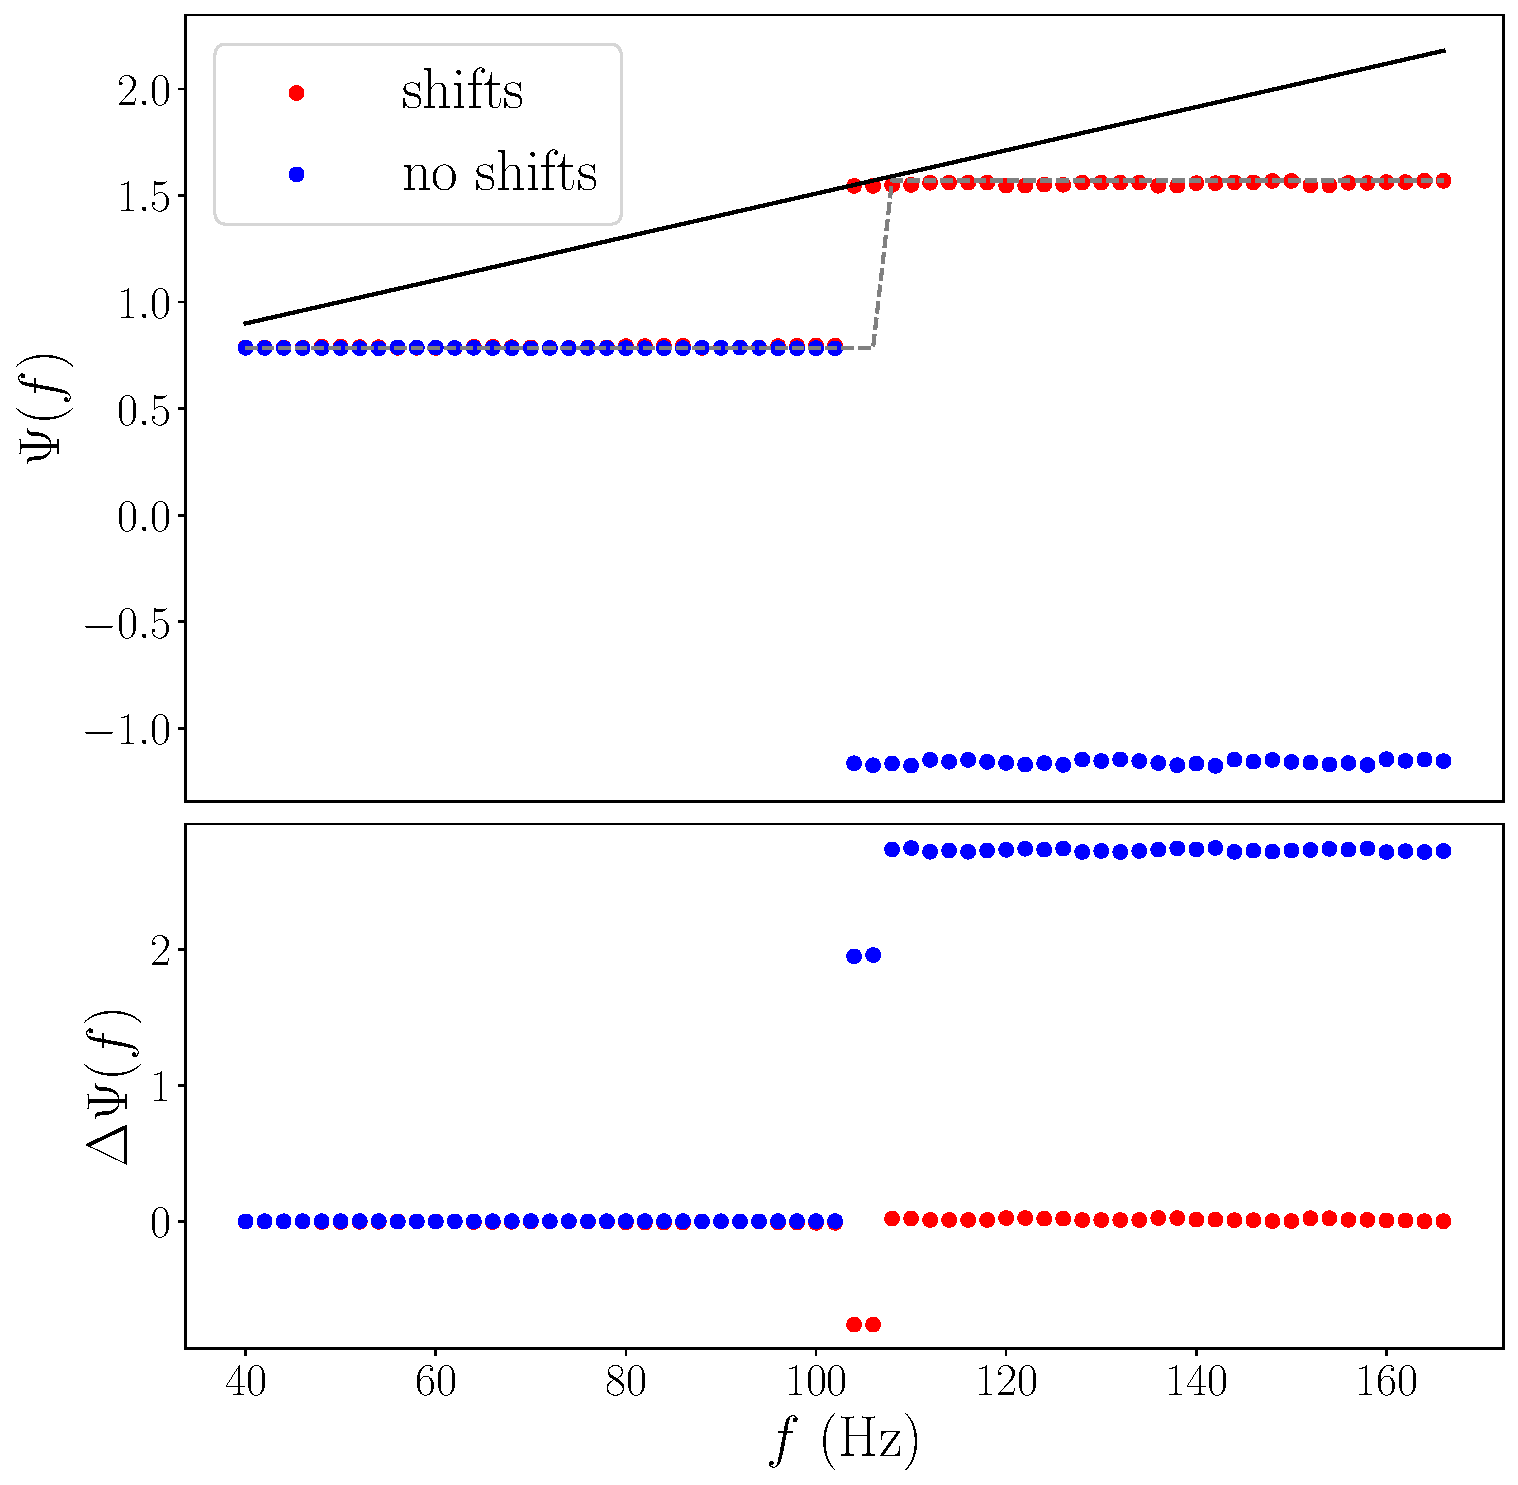
\includegraphics[width=\textwidth]{im/phase_shift_comp_linear_m3}
\caption{Effects of shifted ILs for $\Psi(f) \sim f$ and $m=3$ ($L=6$, 600 epochs, SAM)}
\end{figure}
\end{column}
\begin{column}{0.5\textwidth}
\begin{figure}
\centering 
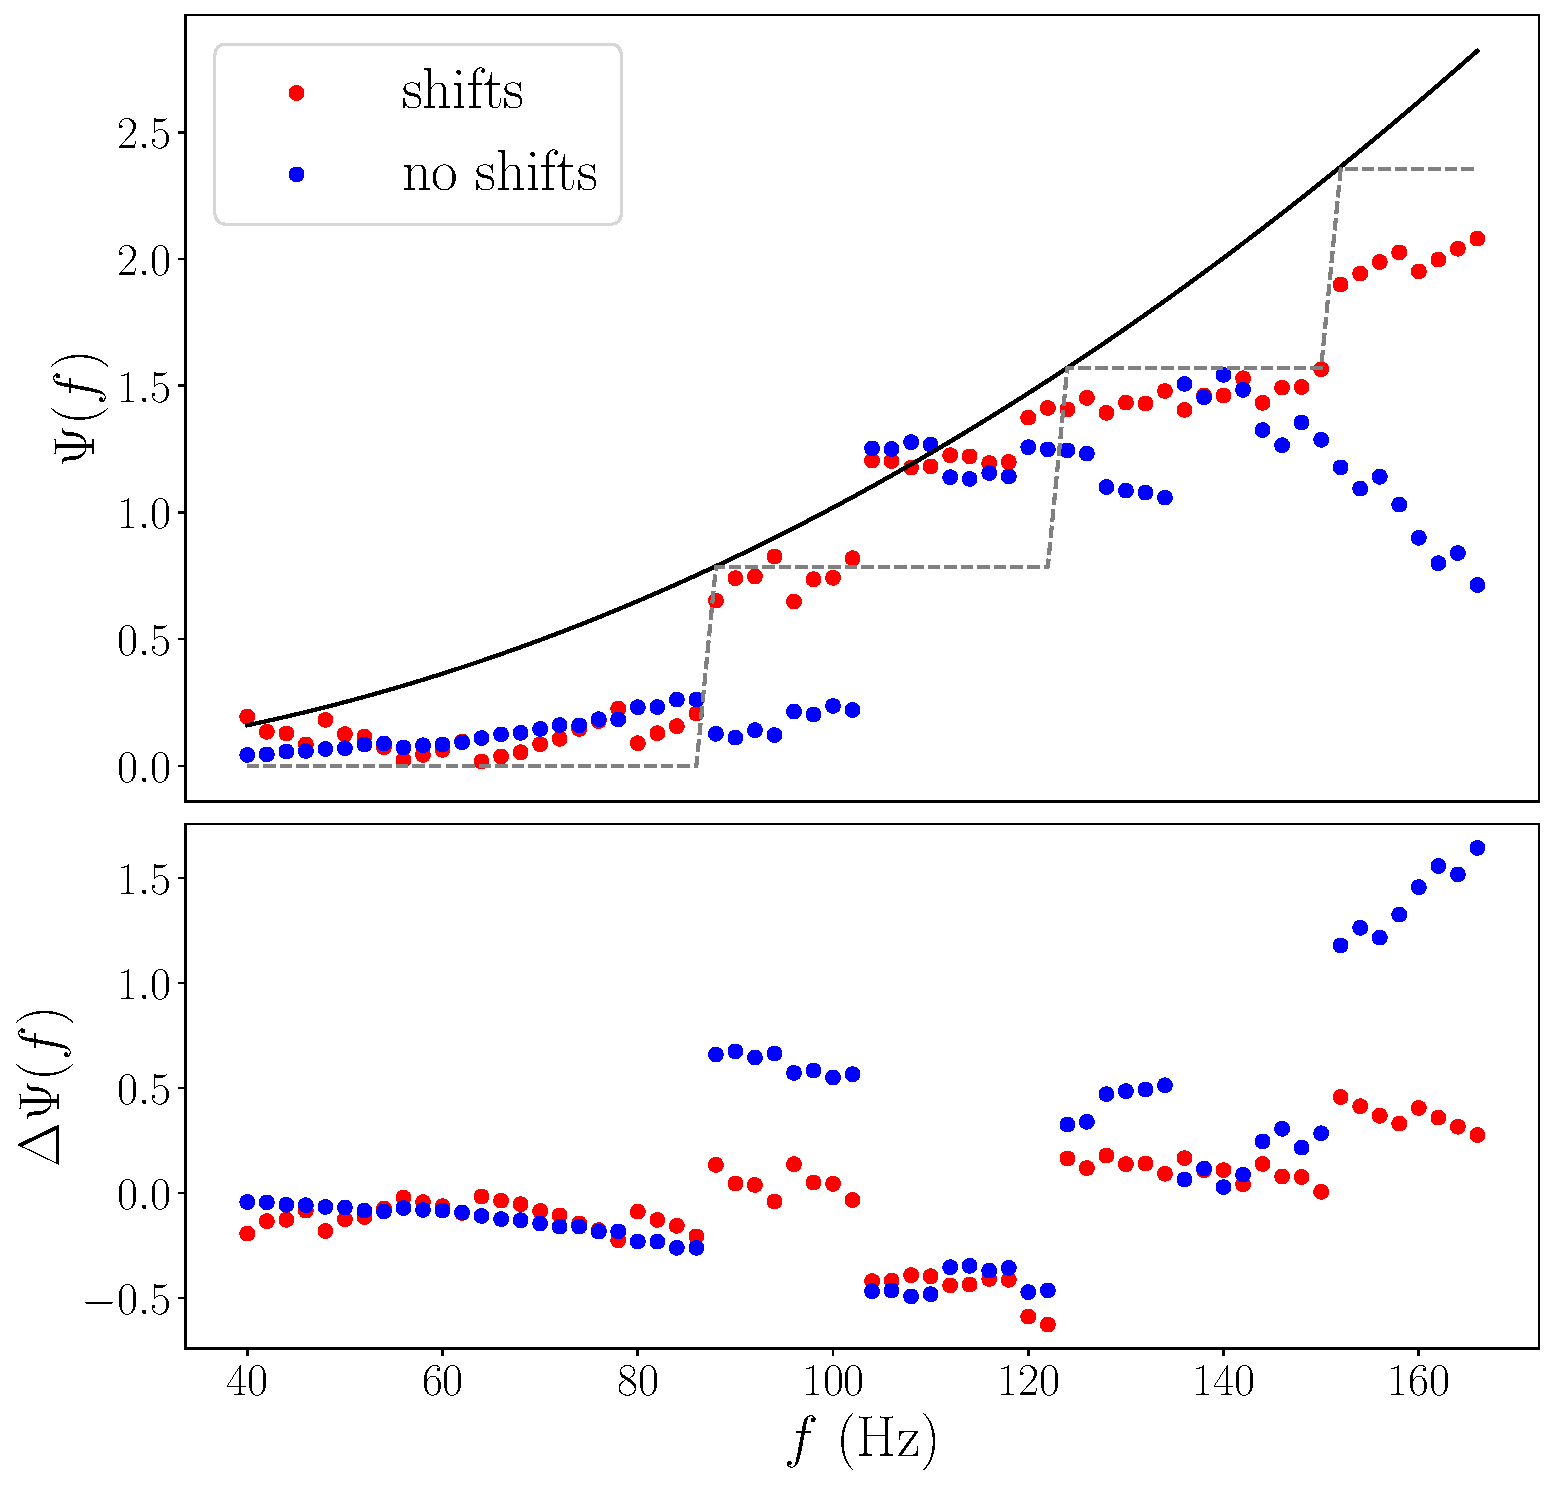
\includegraphics[width=\textwidth]{im/phase_shift_comp_quadratic_m3}
\caption{Effects of shifted ILs for $\Psi(f) \sim f^2$ and $m=3$ ($L=6$, 600 epochs, SAM)}
\end{figure}
\end{column}
\end{columns}
\end{frame}

\begin{frame}
\frametitle{Changing Input Layer Structure}
\begin{columns}
\begin{column}{0.5\textwidth}
\begin{figure}
\centering 
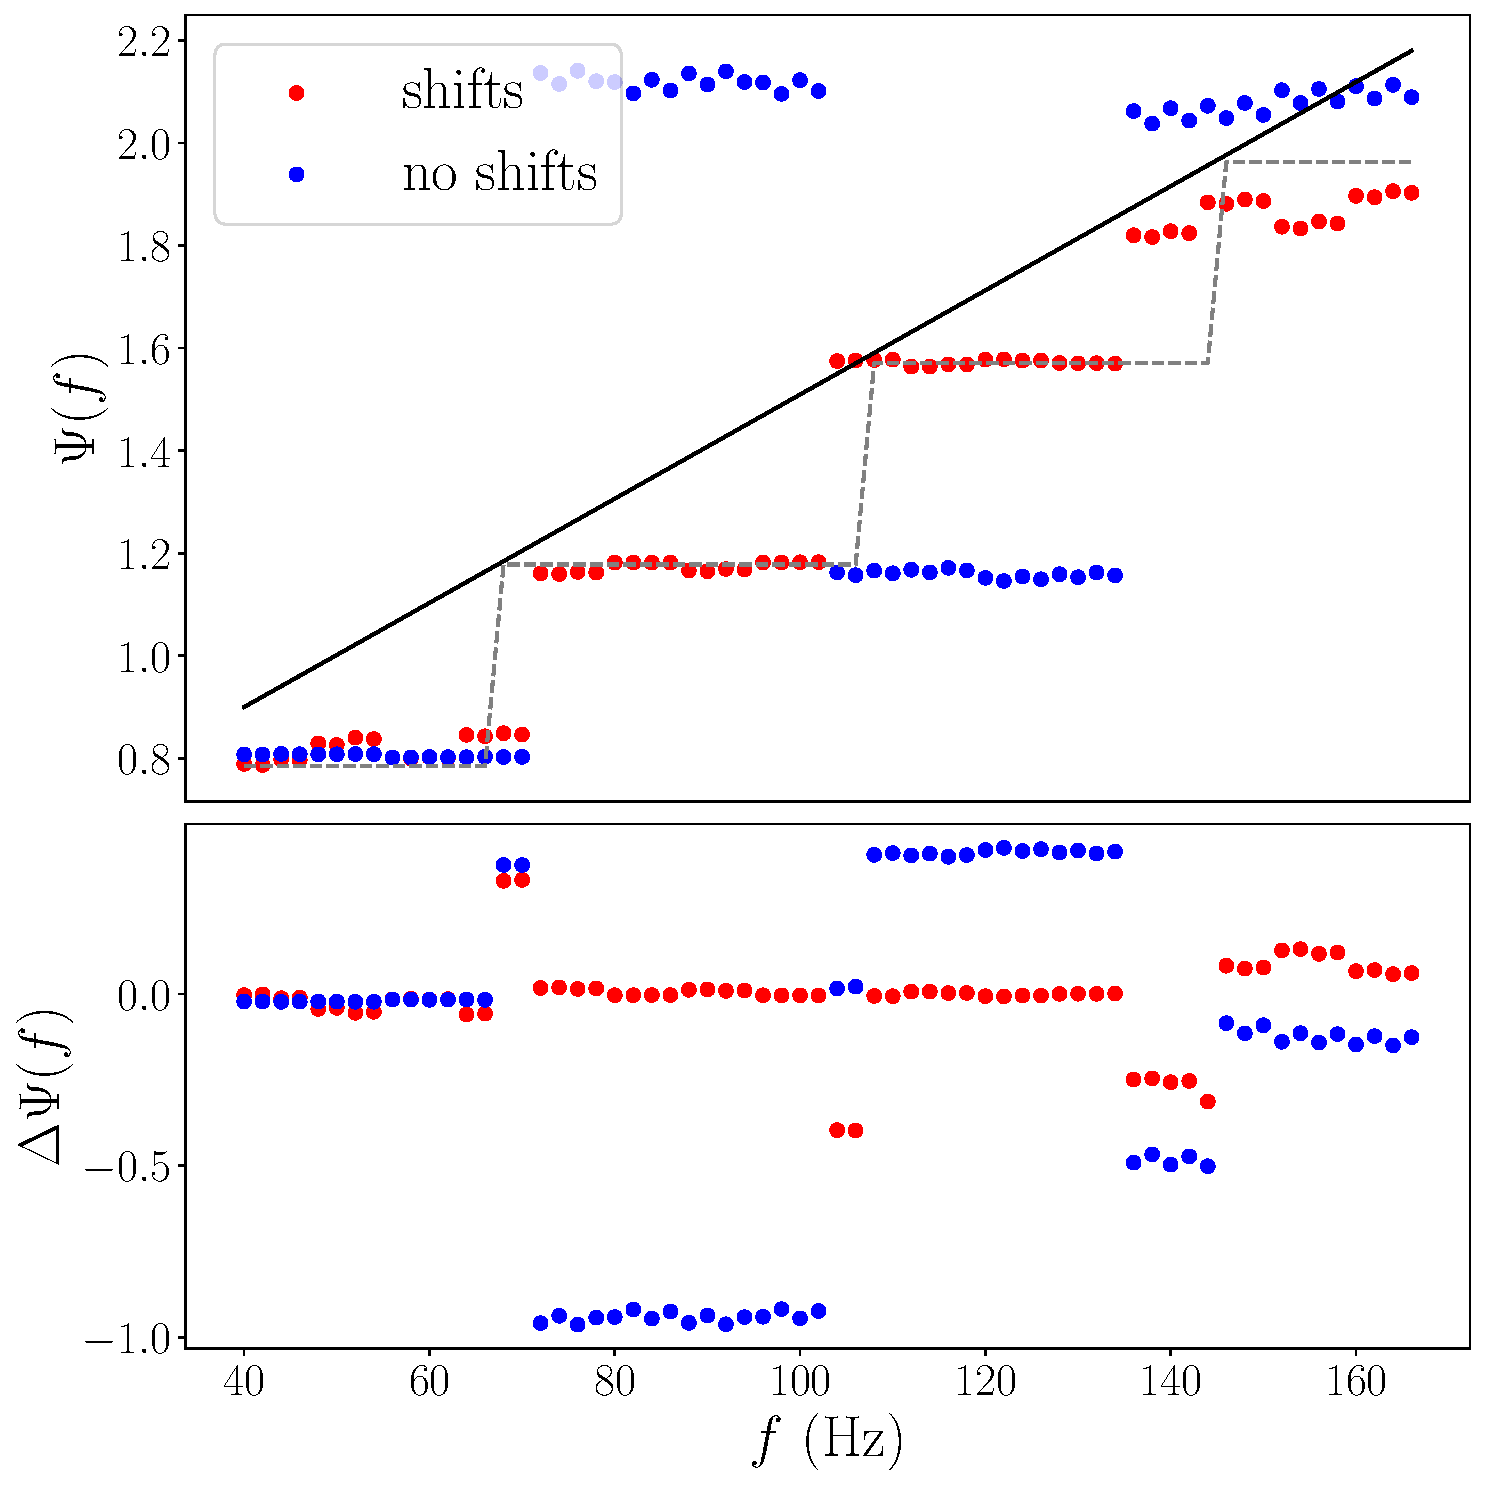
\includegraphics[width=\textwidth]{im/phase_shift_comp_linear_m4}
\caption{Effects of shifted ILs for $\Psi(f) \sim f$ and $m=4$ ($L=6$, 600 epochs, SAM)}
\end{figure}
\end{column}
\begin{column}{0.5\textwidth}
\begin{figure}
\centering 
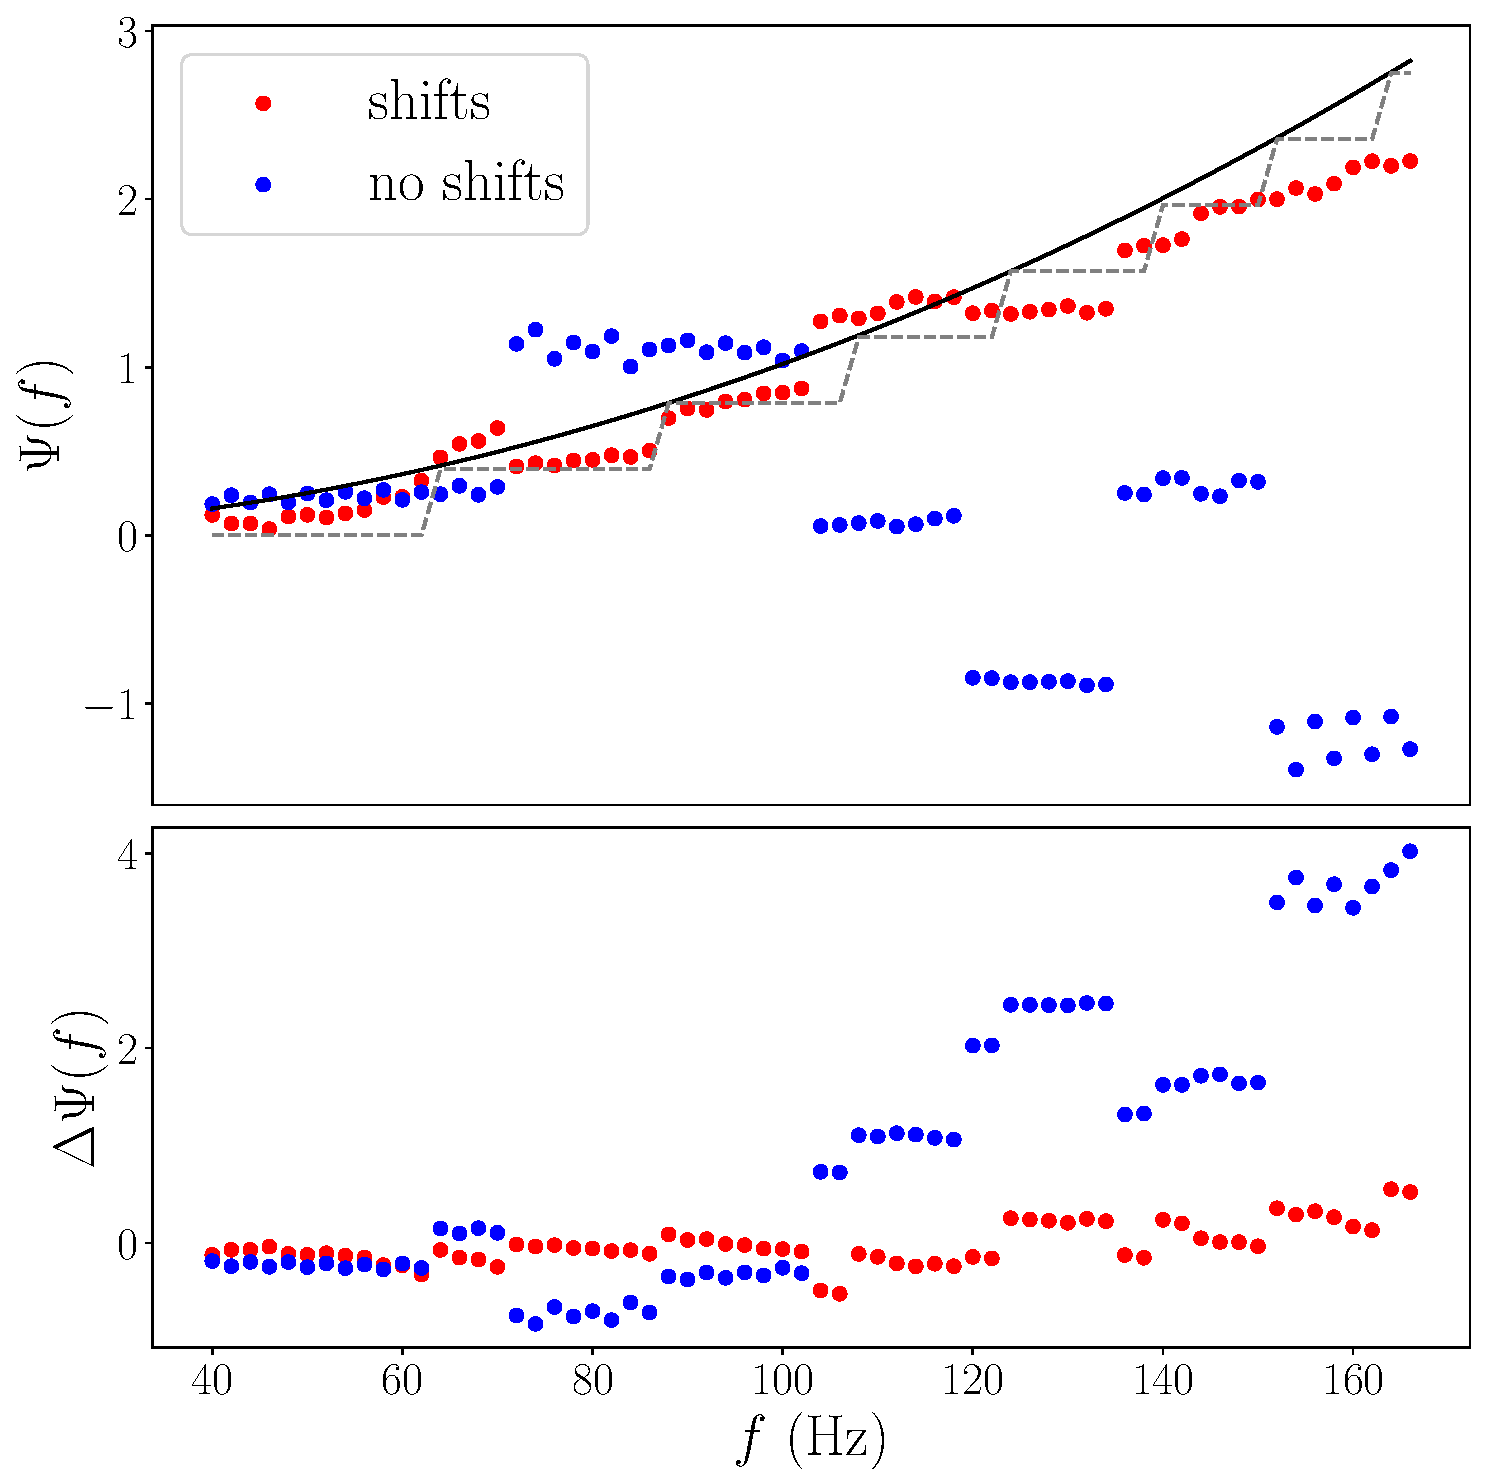
\includegraphics[width=\textwidth]{im/phase_shift_comp_quadratic_m4}
\caption{Effects of shifted ILs for $\Psi(f) \sim f^2$ and $m=4$ ($L=6$, 600 epochs, SAM)}
\end{figure}
\end{column}
\end{columns}
\end{frame}

\begin{frame}
\frametitle{Changing Input Layer Structure}
\begin{columns}
\begin{column}{0.5\textwidth}
\begin{itemize}
\item The data for `no shifts' was obtained by setting  $s=0$ for all ILs instead of incrementing $s$
\item This should be equivalent to last week's circuit structure 
\item However, the `no shifts' results are significantly worse than the results shown last week (\alert{???})
\item Thus, the improvements due to the new IL structure are somewhat exaggerated  
\item Nonetheless, \alert{increased IL connectivity clearly leads to improved performance}
\end{itemize}
\end{column}
\begin{column}{0.5\textwidth}
\begin{figure}
\centering 
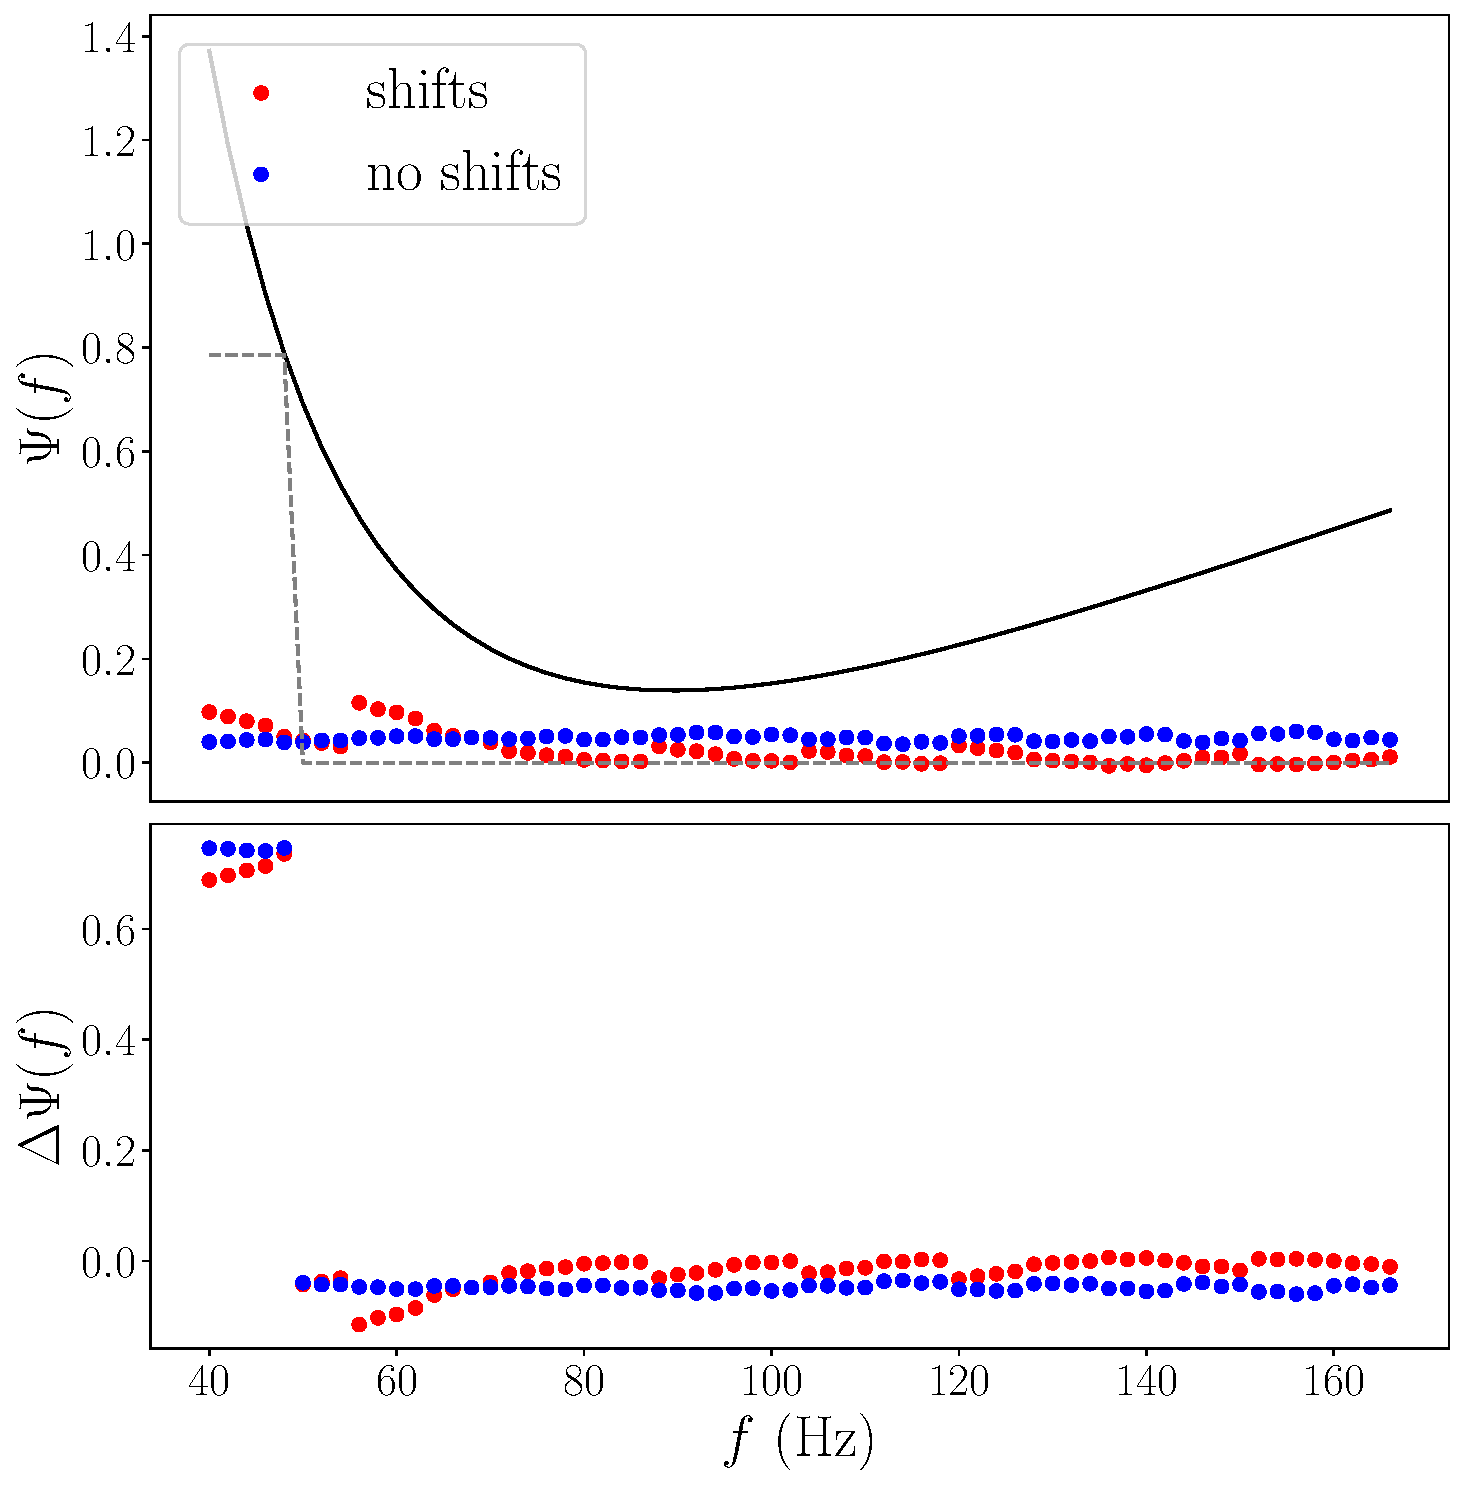
\includegraphics[width=\textwidth]{im/phase_shift_comp_psi_m3}
\caption{Effects of shifted ILs for $\Psi_\text{Hayes2023}$ and $m=3$ ($L=6$, 600 epochs, SAM)}
\end{figure}
\end{column}
\end{columns}
\end{frame}


\section{Fixing Parameters}

\begin{frame}
\frametitle{Fixing Parameters}
\begin{itemize}
\item Implemented the option to \alert{fix parameters for each layer type}
\item This means that each instance of a layer type (IL, AA-CL, NN-CL) uses the same set of parameters 
\item This significantly \alert{reduces the number of trainable parameters} at large $L$
\item Surprisingly, reducing the parameter space \alert{produces no noticeable speed-up} (so-called qiskit primitives, i.e. the sampler, take up roughly 95\% of the computational time)
\end{itemize}
\end{frame}

\begin{frame}
\frametitle{Fixing Parameters}
\begin{columns}
\begin{column}{0.5\textwidth}
\begin{figure}
\centering 
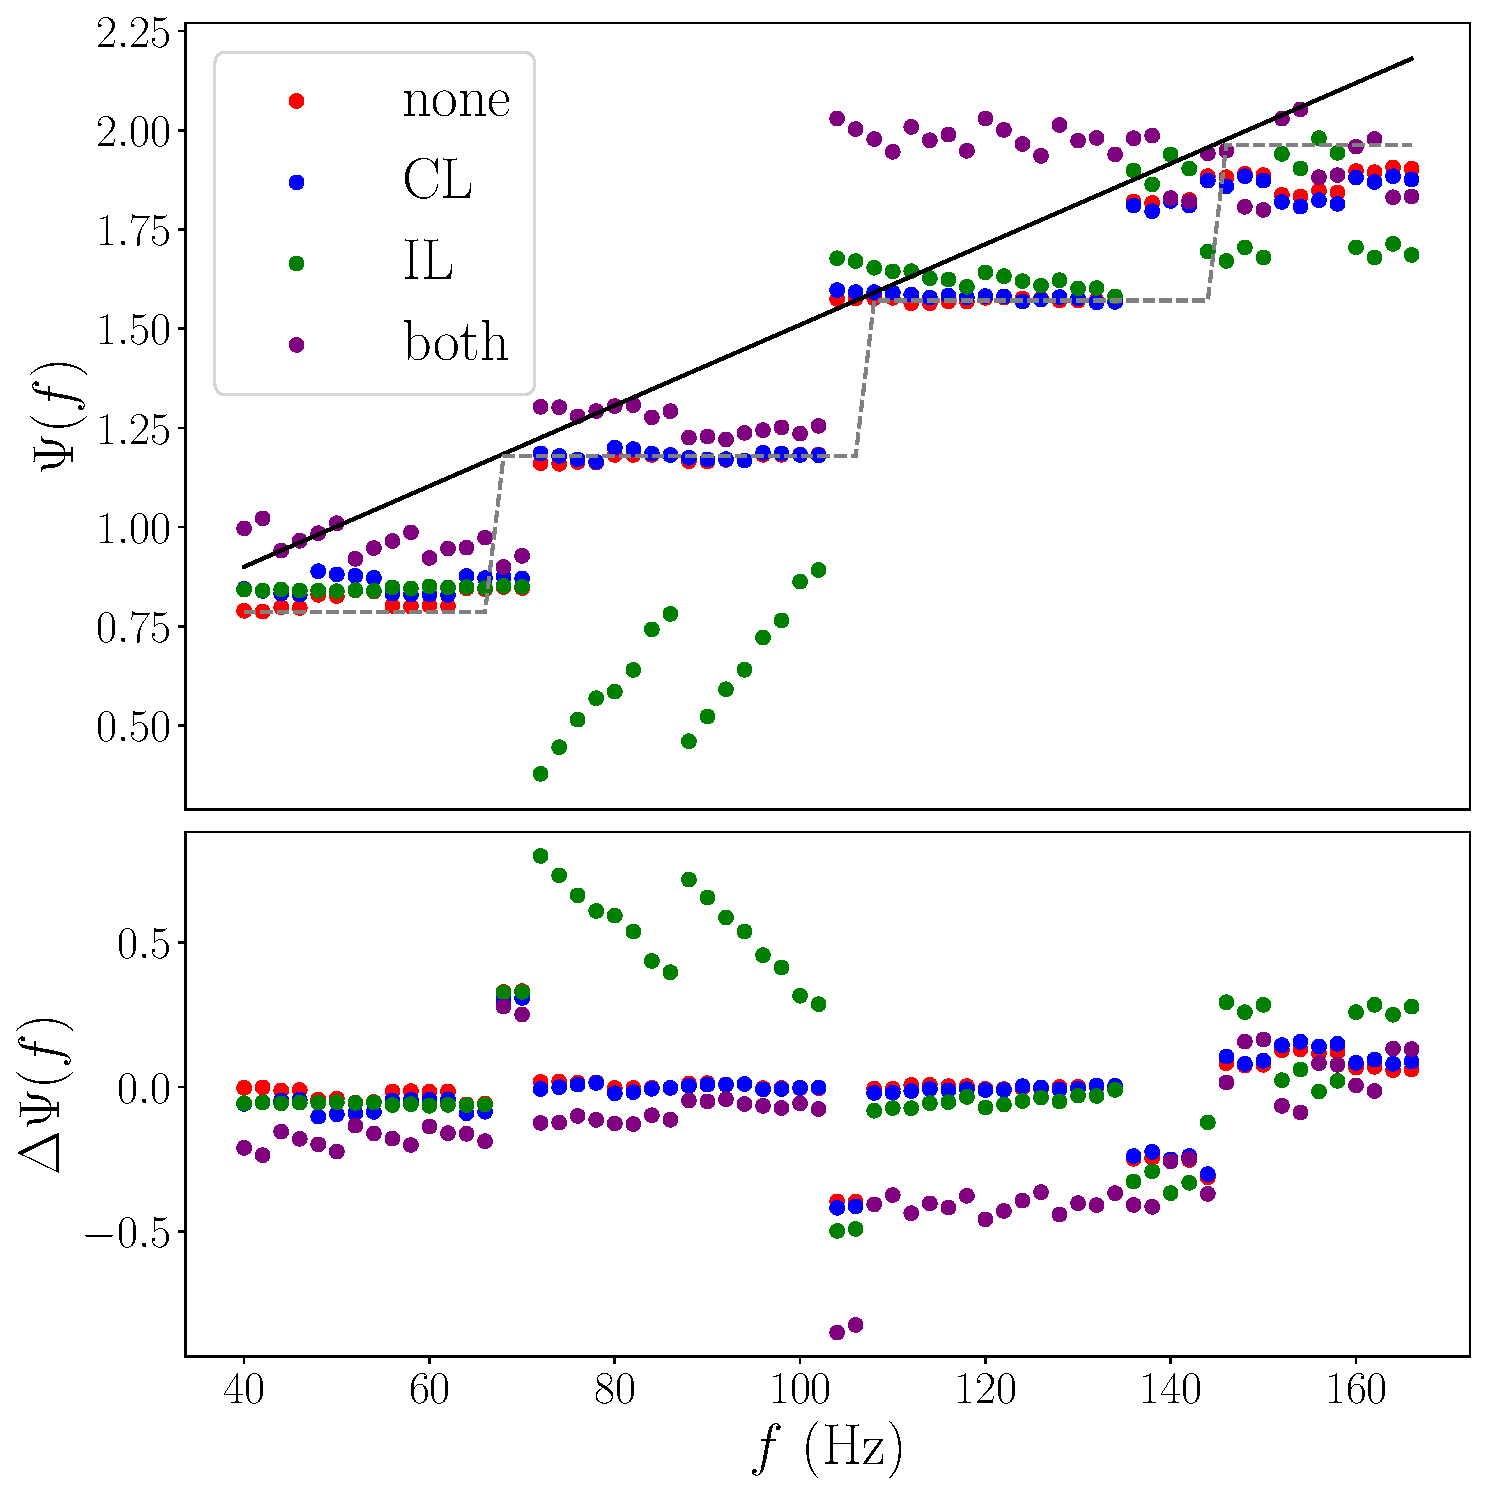
\includegraphics[width=\textwidth]{im/phase_RP_comp_linear_m4}
\caption{Effects of fixing parameters ILs for $\Psi(f) \sim f$ and $m=4$ ($L=6$, 600 epochs, SAM)}
\end{figure}
\end{column}
\begin{column}{0.5\textwidth}
\begin{figure}
\centering 
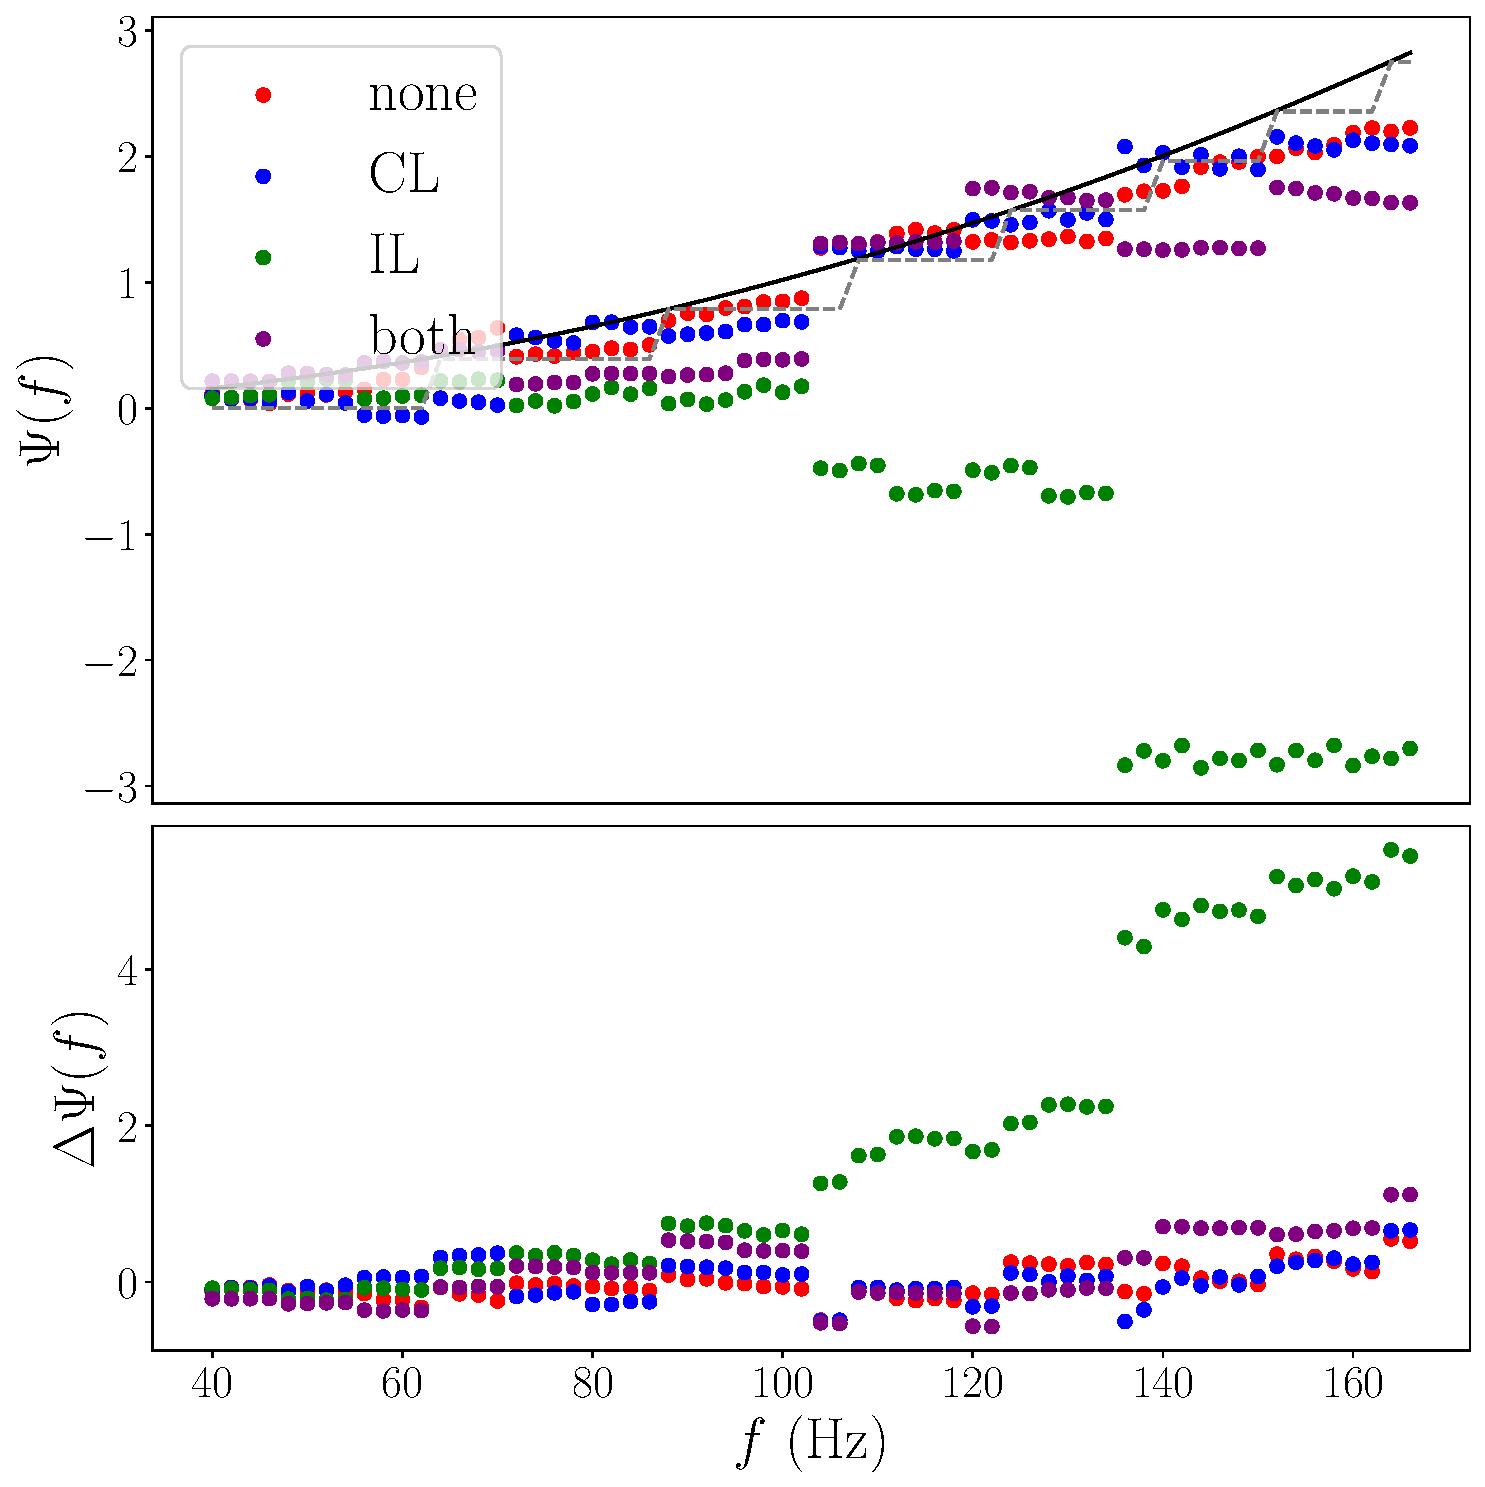
\includegraphics[width=\textwidth]{im/phase_RP_comp_quadratic_m4}
\caption{Effects of fixing parameters for $\Psi(f) \sim f^2$ and $m=4$ ($L=6$, 600 epochs, SAM)}
\end{figure}
\end{column}
\end{columns}
\end{frame}

\begin{frame}
\frametitle{Fixing Parameters}
\begin{itemize}
\item Legend for the plots on the previous slide:
\begin{itemize}
\item `\emph{none}' : no parameters fixed 
\item `\emph{CL}': only CL parameters fixed
\item `\emph{IL}': only IL parameters fixed 
\item `\emph{both}': all parameters fixed  
\end{itemize} 
\item Evidently, keeping parameters fixed leads to (slightly, for `\emph{CL}', or drastically, for `\emph{IL}' and `\emph{both}') \alert{worse performance} 
\item This is likely due to a reduction of the search space 
\item Note that `\emph{IL}' as well as `\emph{both}' lead to \alert{incomplete phase extraction} (formalise this concept!) and hence somewhat meaningless results 
\item Thus, especially taking into account the equivalent computational times, \alert{not keeping parameters fixed yields better results} 
\item These results suggest a particular importance of ILs compared to CLs 
\end{itemize}
\end{frame}

\section{Improving the Loss Function}

\subsection{Preliminary Definitions}

\begin{frame}
\frametitle{Preliminary Definitions}
\begin{itemize}
\item Consider a \alert{computational basis state}, $\ket{j}$, in a $p$-qubit register:
\begin{equation}
\ket{j} = \bigotimes^{p-1}_{\alpha=0} \ket{j_\alpha}, \; \; \; \; \ket{j_\alpha} \in \{\ket{0},\ket{1} \}
\end{equation}
\item Define 
\begin{equation}
j_\alpha \equiv \begin{cases}
0 & \text{if } \ket{j_\alpha}=\ket{0} \\
1 & \text{if }  \ket{j_\alpha}=\ket{1} \\
\end{cases}
\end{equation}
\item Two \alert{digitally encoded binary numbers} can be associated with $\ket{j}$:
\begin{align}
j &\equiv \sum_{\alpha=0}^{p-1} j_\alpha 2^{\alpha} &(0 \leq j \leq 2^p-1 ), \\
j' &\equiv \sum_{\alpha=0}^{p-1} j_\alpha 2^{\alpha-p} &(0 \leq j' \leq 1)
\end{align}
\end{itemize}
\end{frame}

\begin{frame}
\frametitle{Preliminary Definitions}
\begin{itemize}
\item Consider an $n$-qubit \alert{input register} and an $m$-qubit \alert{target register}, denoted with subscripts $i$ and $t$, respectively 
\item A computational basis state of the combined system, $\ket{k}_{i+t}$, can be decomposed into
\begin{equation}
\ket{k}_{i+t} = \ket{j}_i \otimes \ket{l}_t,
\end{equation}
for computational basis states $\ket{j}_i$, $\ket{l}_t$ of the two registers
\item Define 
\begin{align}
\mathsf{input}(\ket{k}_{i+t}) &\equiv \ket{j}_i \\
\mathsf{target}(\ket{k}_{i+t}) &\equiv \ket{l}_t \\
\end{align}
\item A \alert{general state of the two-register system} is then 
\begin{equation}
\ket{z} = \sum^{2^{n+m}-1}_{k=0} z_k \ket{k}_{i+t}
\end{equation}
\end{itemize}
\end{frame}

\begin{frame}
\frametitle{Preliminary Definitions}
\begin{itemize}
\item For training in superposition, the two-register target state is 
\begin{equation}
\ket{y} = \sum_{j=0}^{2^n -1} \frac{1}{\sqrt{2^n}} \ket{j}_i \ket{\Psi'(j)}_t \equiv \sum_{k=0}^{2^{n+m}-1} y_k \ket{k}_{i+t}, 
\end{equation}
with $y_k =0$ if target($\ket{k}_{i+t}$)
\end{itemize}
\end{frame}

\begin{frame}
\frametitle{Preliminary Definitions}
\begin{itemize}
\item FIND GOOD NOTATION FOR ALL THIS !!!
\item THINK ABOUT THIS ALL MORE DEEPLY! MAYBE HAVE TO SWITCH TO WEIGHTED L1/2 LOSS INSTEAD? (WILL)
\end{itemize}
\end{frame}

\begin{frame}
\frametitle{Improving WIM}
\begin{itemize}
\item Recall the definition of \alert{WIM} (\alert{W}e\alert{I}ghted \alert{M}ismatch):
\begin{equation}
\mathsf{WIM}(x,y) =  \left\vert 1 - \sum_{k=0}^{2^{n+m}-1} \tilde{w}_k x_k y_k \right \vert, 
\end{equation}
where
\begin{itemize}
\item $\ket{x} = \sum_{k=0}^{2^{n+m}-1} x_k \ket{k} $ is the output state produced by the QCNN,
\item $\ket{y} = \sum_{k=0}^{2^{n+m}-1} y_k \ket{k} $ is the target state, 
\item $\tilde{w}_k \in \mathbb{R}_+$ are weighting factors 
\end{itemize}
\item .... calculate $w_k$
\item $\tilde{w}$
\end{itemize}
\end{frame}

\section{Results}

\begin{frame}
\frametitle{Results}
Show phase encoding with improved methods 
show the full waveform [new frame]
\end{frame}

\section{Next Steps}

\begin{frame}
\frametitle{Next Steps}
\begin{itemize}
\item formalise and investigate `completeness of phase extraction' 
\item look into adding more ILs compared to CLs ?
\end{itemize}
\end{frame}



\end{document}